% DOCUMENT
\documentclass[oneside,14pt,a4paper]{extreport}

% LANGUAGE
\usepackage[T2A]{fontenc}
\usepackage[utf8]{inputenc}
\usepackage[english, ukrainian]{babel}

% VARIABLES
\newcommand \labno    {1}
\newcommand \course   {Візуалізація даних}
\newcommand \group    {310}
\newcommand \lecturer {Бойко Наталія Іванівна}
\newcommand \theme    {Аналіз даних	та статистичне виведення}
\newcommand \purpose  {[Мета звіту]}

% PACKAGES
\usepackage{amssymb}
\usepackage{amsmath}
\usepackage{multirow}
\usepackage{pgfplots}

% GEOMETRY
\usepackage{geometry}
\geometry{left   = 2.5cm}
\geometry{right  = 1cm}
\geometry{top    = 2cm}
\geometry{bottom = 2cm}
\renewcommand {\baselinestretch} {1.5}
\setlength\parindent{1cm}

% IMAGES
\usepackage{graphicx}
\usepackage{indentfirst}
\graphicspath{ {./imgs/} }

% FOOTER
\usepackage{scrpage2}
\ifoot[]{}
\cfoot[]{}
\ofoot[\pagemark]{\pagemark}
\pagestyle{scrplain}

% CHAPTERS

\newcommand\Section[1]{
 \refstepcounter{section}
 \section*{
  \arabic{section}. #1}
}

\newcommand\Subsection[1]{
 \refstepcounter{subsection}
 \section*{
  \arabic{section}.\arabic{subsection}. #1}
}

\sloppy
\begin{document}
\begin{titlepage}

\centering
 \textbf{
  МІНІСТЕРСТВО ОСВІТИ І НАУКИ УКРАЇНИ \\
  НАЦІОНАЛЬНИЙ УНІВЕРСИТЕТ \flqq{}ЛЬВІВСЬКА ПОЛІТЕХНІКА\frqq{}
 }

\vspace{1.5cm}
 \textbf{
  Інститут комп'ютерних наук та інформаційних технологій \\
  Кафедра систем штучного інтелекту
}

\vspace*{\fill}

  {\textbf{Лабораторна робота №\labno}
   \par}
  {З курсу \flqq\course\frqq \par}

\vspace{1cm} \theme

\raggedleft\vfill

 {\textbf{Виконав:} \par}
 {ст. гр. КН-\group \par}
 {Бікєєв Андрій \par}

\vspace{1cm}

 {\textbf{Викладач:} \par}
 {\lecturer \par}

\vspace{1cm}

\centering {Львів -- \the\year \par}

\end{titlepage}

\Section{Умова завдання}
\begin{enumerate}
\item Завантажити дані та дослідити їх.
\item Переглянемо перші шість, перші п'ятнадцать та останні шість рядків з наших даних.
\item Дізнатися, яка кількість квартир продається у кожному місті згідно до нашого датасету.
\item Побудуємо стовпчикові діаграми для:
	\begin{enumerate}
	\item кількості кімнат
	\item змінної площа
	\item розподіл квартир, які продаються за загальною площею
	\end{enumerate}
\item Побудувати графік розсіювання, а саме залежності ціни від загальної площі.
\item Побудувати графік розподілу цін по містах.
\end{enumerate}

\Section{Хід роботи}

Для лабораторної роботи я використав бібліотеки:
\begin{itemize}
\item pandas - для імпорту .csv файлу у датафрейм.
\item matpotlib - для будування графіків.
\item seaborne - для будування більш "складних" графіків.
\end{itemize}

\Subsection{Імпортування бібліотек і даних}
\small
\begin{verbatim}
import pandas as pd
import matplotlib.pyplot as plt
import numpy as np
import seaborn as sns

data = pd.read_csv("flats.csv", sep = ',', decimal=',')
data.columns = [col.replace('"', '') for col in data.columns]
\end{verbatim}

\Subsection{Знаходження кількості вимірів, відображення і огляд інформації}
\begin{figure}[!htb]
 \centering
 
\includegraphics[scale=1.0]{mission_1}
 \caption{Завдання} 
\end{figure}

\small
\begin{verbatim}
print(data.shape)

print(data.head(6))
print(data.head(15))
print(data.tail(6))

print(data.columns)
\end{verbatim}

\begin{figure}[!htb]
 \centering
 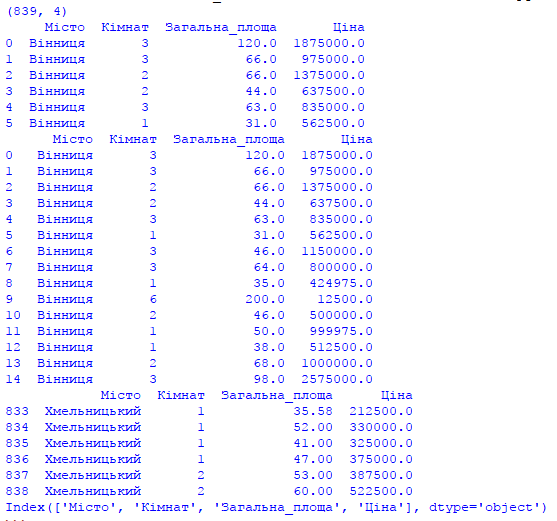
\includegraphics[scale=1.0]{result_1}
 \caption{Результат виконання} 
\end{figure}

\newpage
\Subsection{Перевірка та попередній аналіз даних}
\begin{figure}[!htb]
 \centering
 
\includegraphics[scale=1.0]{mission_2}
 \caption{Завдання} 
\end{figure}

\small
\begin{verbatim}
print(len(data.columns))
print(len(data.filter(items="Місто")))
print(len(data[(data.Місто == "Одеса") & (data.Кімнат == 3)]))

data["Загальна_площа"] = data["Загальна_площа"].str.replace(
    ',', '.'
).astype(float)
newdata = data[(data.Місто == "Львів") & (data.Кімнат == 1)]
print(newdata["Загальна_площа"].median())
\end{verbatim}

\begin{figure}[!htb]
 \centering
 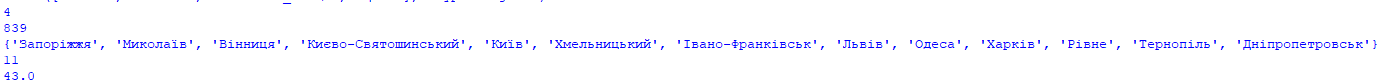
\includegraphics[scale=1.0]{result_2}
 \caption{Результат виконання} 
\end{figure}

Як бачимо, ні, не всі записи у наборі даних flats є містами, наприклад Києво-Святошинський є районом Київської області, а не містом. Це може привести до спотворення даних, адже ці записи складають приблизно 2.2\% від усіх записів(19/839).

\Subsection{Побудова діаграм, та їх аналіз}
\begin{enumerate}
\item \textbf{Стовпчикова діаграма за кількістю кімнат.}

\small
\begin{verbatim}
print(len(data.columns))
print(len(data.filter(items="Місто")))
print(len(data[(data.Місто == "Одеса") & (data.Кімнат == 3)]))

data["Загальна_площа"] = data["Загальна_площа"].str.replace(
    ',', '.'
).astype(float)
newdata = data[(data.Місто == "Львів") & (data.Кімнат == 1)]
print(newdata["Загальна_площа"].median())
\end{verbatim}

\newpage
\begin{figure}[!htb]
 \centering
 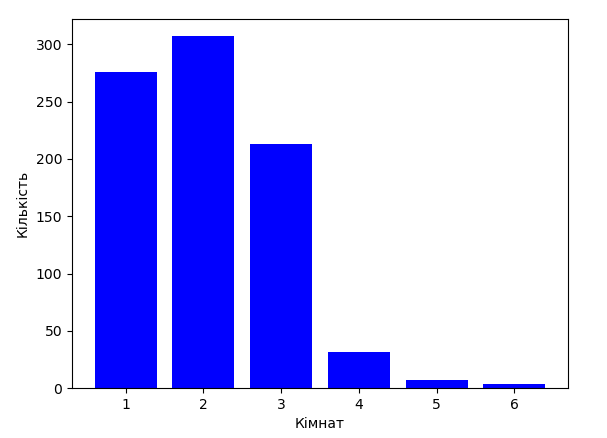
\includegraphics[scale=1.0]{graph_1}
 \caption{Діаграма Стовпчикова "Кількість кімнат"} 
\end{figure}

За допомогою діаграми, бачимо, що кількість кімнат у квартирах, які продають, розподілена нерівномірно, наприклад найчастіше зустрічаються квартири двухкімнатні(300 записів), що є модою нашої вибірки. Рідше всього продають квартири 6-и кімнатні, що певно зумовлено низьким попитом на такого роду квартири.

\item \textbf{Стовпчикова діаграма за загальною площею.}

\small
\begin{verbatim}
values = data.groupby('Загальна_площа').size().reset_index(name='Кількість')
x_ax = values['Загальна_площа'].tolist()
y_ax = values['Кількість'].tolist()
plt.bar(x_ax,y_ax, color='r')
plt.xlabel('Загальна_площа')
plt.ylabel('Кількість')
plt.show()
\end{verbatim}

\begin{figure}[!htb]
 \centering
 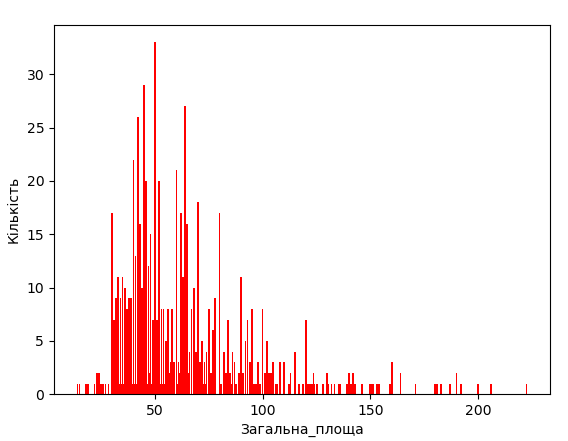
\includegraphics[scale=1.0]{graph_2}
 \caption{Діаграма Стовпчикова "Загальна площа"} 
\end{figure}

На діаграмі за загальною площею можна побачити схожий розподіл на розподіл діаграми за кількістю кімнат, адже їх кількість корелює з площею, і деякі чинники в цих випадках спільні.

\item \textbf{Графік розподілу квартир, за загальною площею}

\small
\begin{verbatim}
x = data['Загальна_площа']
x.plot('hist', bins=[i for i in range(0,251,25)], align='mid', color='steelblue')
plt.xlabel('Загальна_Площа')
plt.ylabel('Кількість')
plt.show()
\end{verbatim}

\newpage
\begin{figure}[!htb]
 \centering
 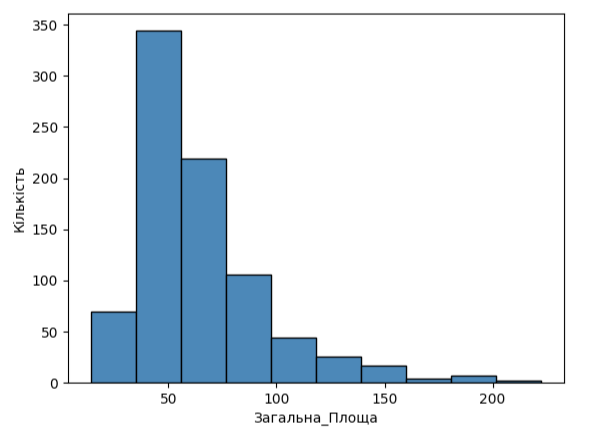
\includegraphics[scale=1.0]{graph_3}
 \caption{Графік розподілу "Загальна площа"} 
\end{figure}

\item \textbf{Графік розсіювання - залежність між ціною і загальною площею}

\small
\begin{verbatim}
x = data['Загальна_площа']
y = data['Ціна']
plt.scatter(x, y, 3, c='g')
plt.yticks(np.arange(0, 12500001, 2500000))
plt.xticks(np.arange(0, 201, 50))
plt.xlabel('Загальна_площа')
plt.ylabel('Ціна')
plt.show()
\end{verbatim}

\newpage
\begin{figure}[!htb]
 \centering
 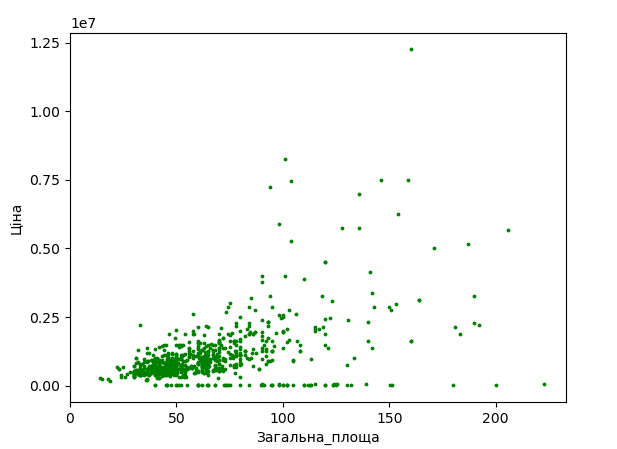
\includegraphics[scale=1.0]{graph_4}
 \caption{Графік розсіювання "Ціна і загальна площа"} 
\end{figure}

На цьому графіку окрім тренду більша площадь = більша ціна можна побачити аномальну лінію ціна 0, що певно є результатом незаповнених даних про ціну квартири на оголошеннях.

Деякі інші аномалії певно спричинені іншими залежностями ціни квартири, наприклад її розташуванням, або "видом з вікна".

\item \textbf{Графік розподілу цін по містах}

\small
\begin{verbatim}
plt.figure(figsize=(15, 15))
ax=sns.boxplot(y='Місто', x="Ціна",orient='h', data=data, linewidth=2)
plt.show()
\end{verbatim}

\newpage
\begin{figure}[!htb]
 \centering
 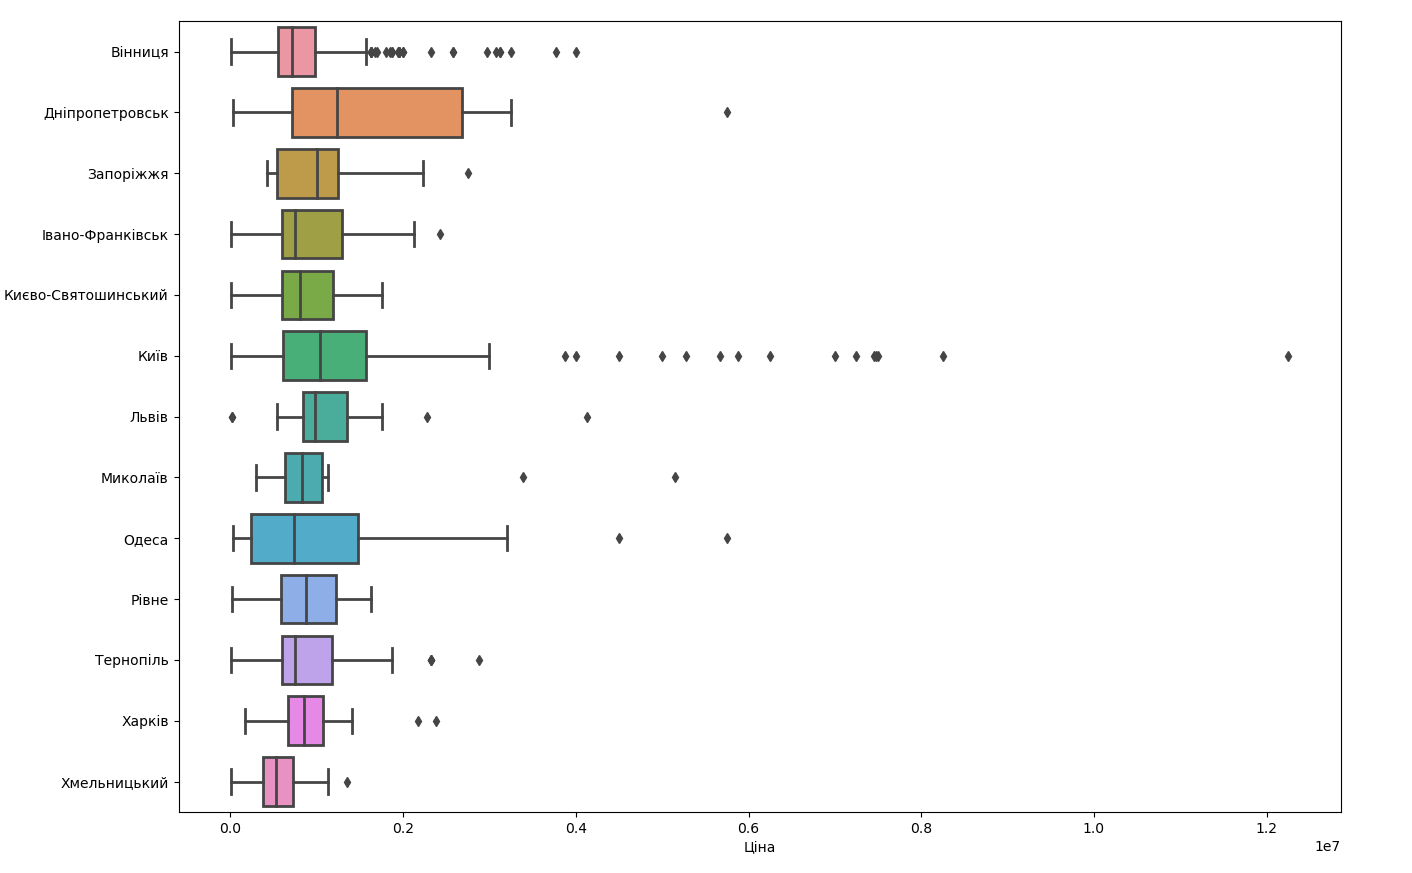
\includegraphics[scale=1.0]{graph_5}
 \caption{Графік розподілу "Ціни по містах"} 
\end{figure}

На цьому графіку можна помітити, що найбільший розкид у Одесі, Києві, та Дніпропетровську. Найбільше аномалій у Києві, що певно спричинено підвищенним попитом на квартири у місті-столиці, а також більша наявність "великих" квартир у виборці(Які в свою чергу продаються дорожче).

\end{enumerate}

\Section{Висновки}

Виконуючи цю лабораторну роботу я навчився зчитувати .csv файли, будувати графіки і діаграми з отриманих даних, а також аналізувати їх.

\end{document}
